\graphicspath{{parte_2/Interfaz de usuario}}

\renewcommand{\chaptername}{interfaz de usuario}

\chapter{Interfaz De usuario} % \label{cap:int_user}
\markright {Interfaz de usuario	}
\begin{center}
	\begin{tcolorbox}[colback=gray!5!white, %Color del fondo
		colframe=blue!75!black,
		title= \center{\Large{resumen}} ]
		Se van a definir las interfaces sobre las computadoras de la institución. Estas interfaces, se basan en software existente. Para seleccionar las interfaces, se realiza una comparación de todos estos. Luego de esto, se va a mostrar cómo realizar la configuración de los dos software seleccionados.   
	\end{tcolorbox}
\end{center}    



\section{introducción}
En esta sección, analizamos los programas que son capaces de mostrar las posiciones de los satélites en tiempos real. Luego de un análisis, se seleccionan dos de estos mismos. Los programas existentes deben tener capacidad de enviar las posiciones de los satélites usando la red local de la institución. Luego del análisis de los programas, se muestran cuáles deben ser los pasos a seguir para poder configurar dichos programas.  

\section{Interfaz de Usuario}

La figura \ref{fig:fig_ssgen}, se observa que hay estaciones de trabajo. En esta sección, definimos el software de seguimiento de satélites, para las estaciones de trabajo del lugar. Algunos de los software que se analizan fueron obtenidos desde la página web de la AMSAT (asociación mundial de satélites de radioaficionados),y otros desde la investigación a través de Internet. 
Los distintos programas que se analizan son: 
\begin{itemize}
	\item Gpredict 
	\item Stelarium 
	\item Orbitron 
	\item Celestia 
	\item Pass 
\end{itemize}
Hay que destacar, que todos estas aplicaciones, requieren la ubicación del usuario(en este caso, de la antena), en sistemas de coordenadas terrestres(latitud y longitud del lugar, con su respectivo signo). 


\subsection{Orbitron}
Este software permite la ubicación de satélites en tiempo real, permite simulaciones donde se pueden observar el día y la hora aproximada de llegada del satélite al plano del horizonte(ver capítulo \ref{cap:sist_cord}) donde se encuentre la antena. 
Además, permite que observar la posición del sol y la luna en tiempo real. 

\begin{figure}[ht]
	\centering
	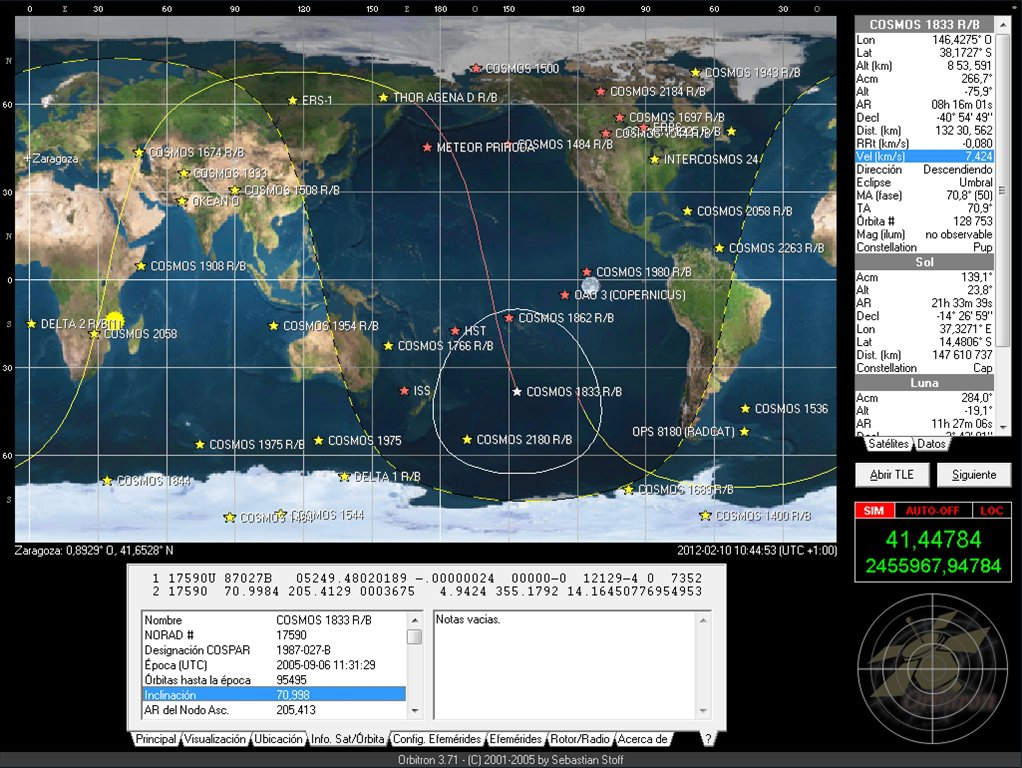
\includegraphics[scale=0.4]{orbitron}
	\caption{Captura de pantalla del software Orbitron }
\end{figure}

Como contra de este software, es que no permite realizar el seguimiento de estrellas, y no puede conectarse a la red, para enviar estos datos a través de la red local. Solo tiene conexión con los puertos(puertos USB) de la PC para obtener los datos. Para poder enviar estos datos, a través de la red, se debe simular un puerto virtual, obtener esos datos, y enviarlos a través de la red local. Es decir, requiere un programa que haga de intermediario. 

\subsection{Stellarium} 
El software stellarium, posee un seguimiento en tiempo real de estrellas, y está pensado para realizar el seguimiento usando telescopios. Tiene distintos módulos, lo que lo hacen personalizable. Tiene soporte para estrellas, y satélites. Estos datos, pueden enviarse a través de la red, para que los reciba un telescopio, y realice el apuntado del telescopio. Existen pluggins, de este software, que permiten enviar las coordenadas a dispositivos mediante la red. Una imagen del software puede visualizarse en la siguiente figura:% \ref{fig:stelarium_init}  

\begin{figure}[ht]
	\centering
	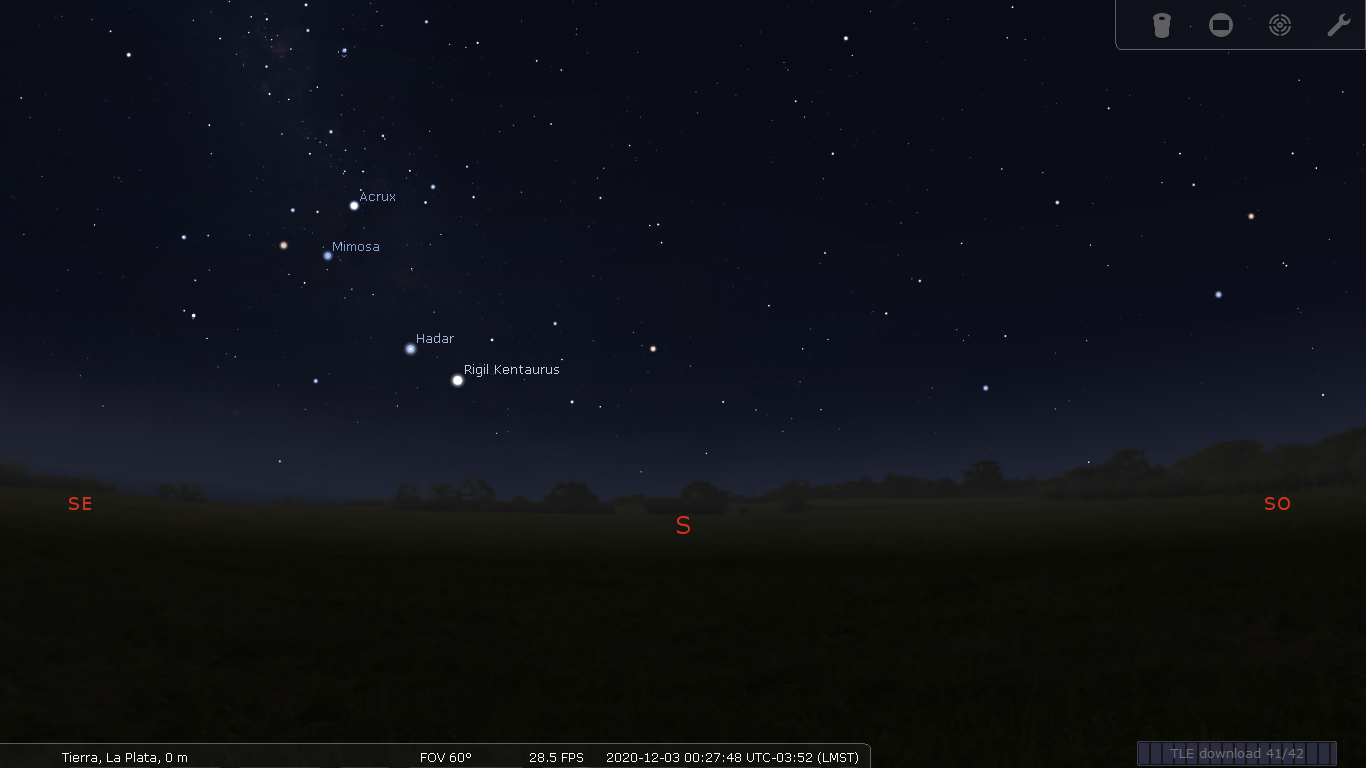
\includegraphics[width=\linewidth,height= 5.6cm]{stellarium}
	\caption{Imagen al abrir el software Stellarium }
	\label{fig:stelarium_init}
\end{figure}




\subsection{Celestia} 
Celestia es un software, que permite realizar ``viajes'' a las estrellas. Este software tiene un fin educativo, puede realizar algunas simulaciones, y se puede viajar al ``espacio a donde uno desee''. Este software no posee ningún tipo de comunicación con el exterior. 
\begin{figure}[ht]
	\centering
	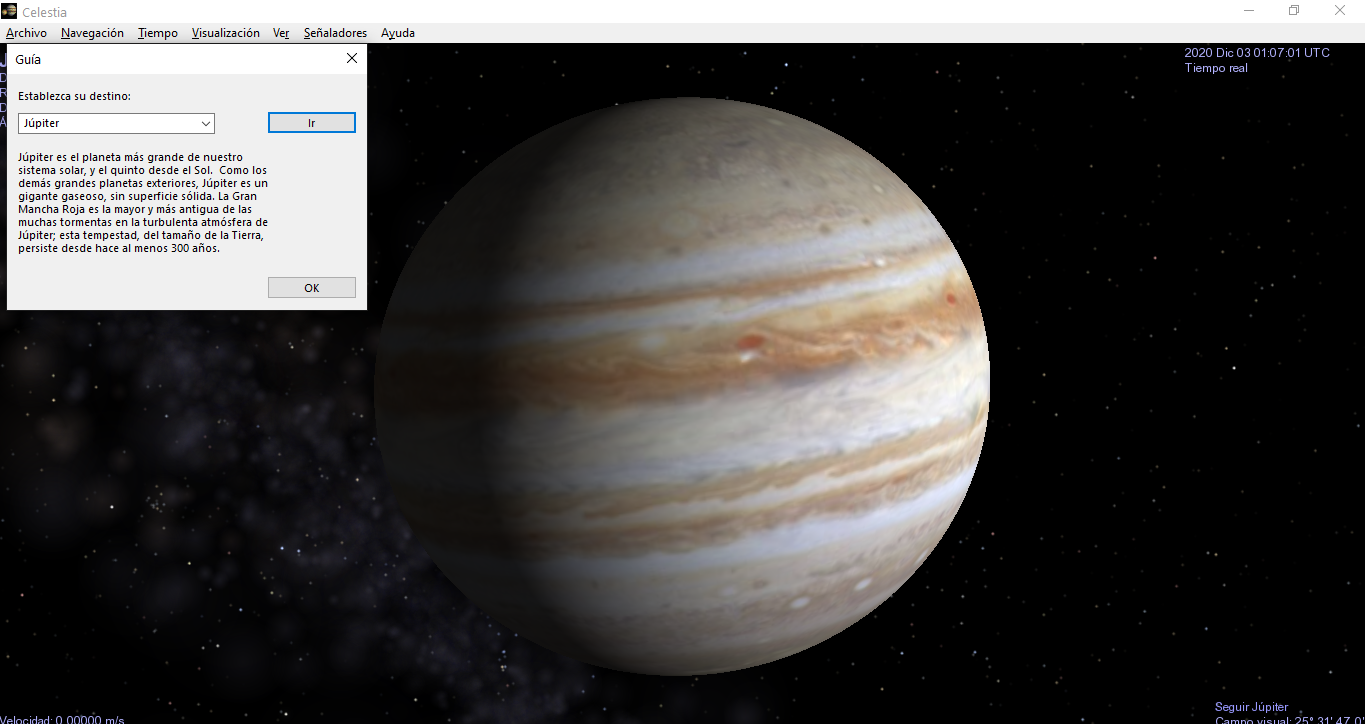
\includegraphics[scale=0.3]{celestia}
	\caption{Viaje a júpiter a través de celestia}
\end{figure}



\subsection{Pass}
Pass no es una aplicación para PC en sí. Es una página web con todos los satélites encima de un mapa. La página es http://amsat.org.ar/pass. La captura de pantalla se muestra en la siguiente figura:% \ref{fig:iu_pass}.
\begin{figure}[ht]
	\centering
	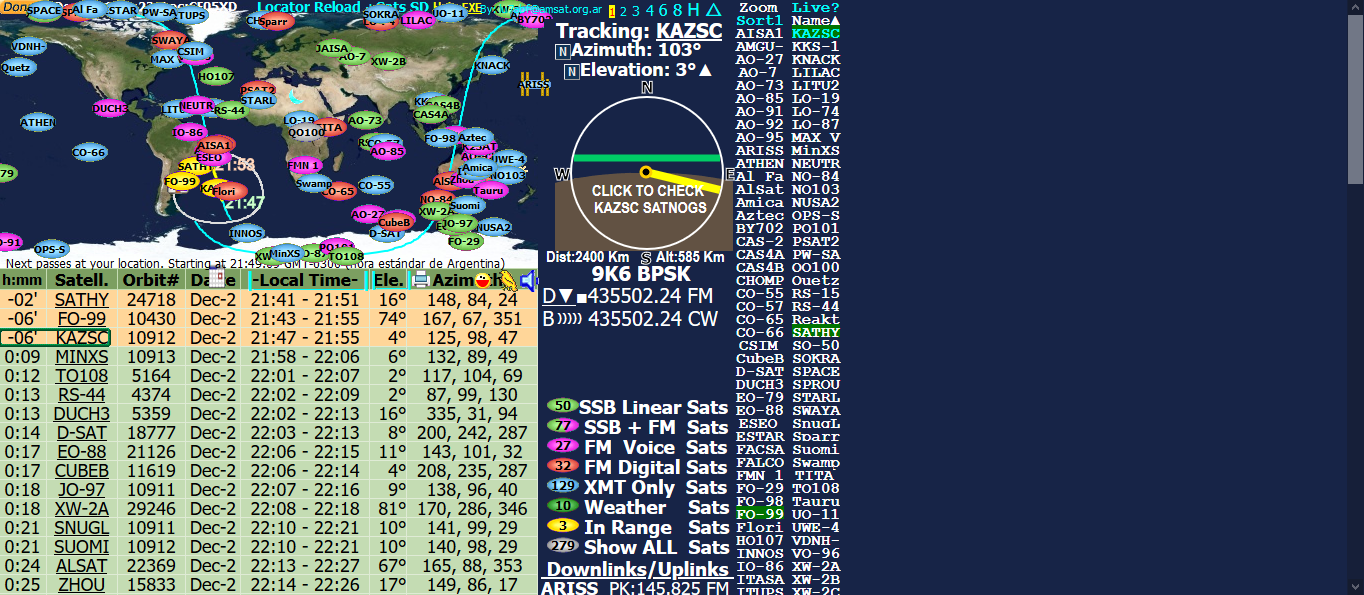
\includegraphics[width=\linewidth, height= 6cm]{pass}
	\caption{Captura de pantalla de la página http://amsat.org.ar/pass }
	\label{fig:iu_pass}
\end{figure}

Éste software, obtiene la geolocalización a partir de la conexión a Internet. A partir, de ellas, obtiene la orientación de la antena. Debido a que obtiene las coordenadas a partir de la conexión a Internet, se tiene un error en el apuntamiento de la antena, ya que estas coordenadas están desfasadas respecto a las reales.    

\subsection{Gpredict}

El software Gpredict es un software que muestra en tiempo real las ubicaciones de los satélites dentro de un mapa, que permite, la configuración de sistemas receptores y sistemas de rotación para antenas. El mismo es libre, su código fuente está disponible en Internet, como así su programa compilado, el mismo puede usarse en Windows y Linux. Este, provee una base de datos de satélites, y se actualiza con la frecuencia que se configure. Además, soporta envió de datos mediante el uso de una red local, configurando sus parámetros. Una captura de pantalla puede verse en la siguiente figura:  %\ref{fig:iu_gpredict}.

\begin{figure}[h]
	\centering
	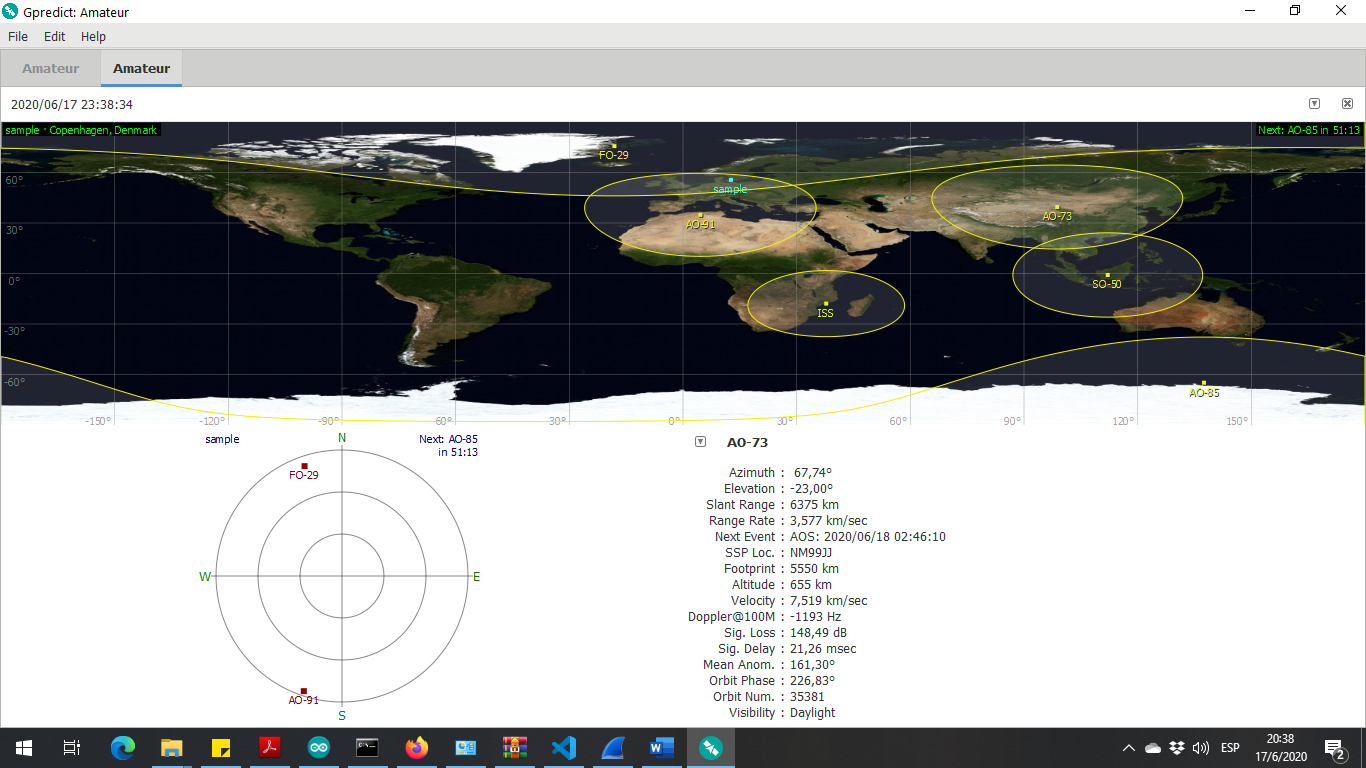
\includegraphics[width=\linewidth,height=7cm]{gpredict}
	\caption{Captura de pantalla del software Gpredict}
	\label{fig:iu_gpredict}
\end{figure}


\section{Comparativa de interfaces y selección del software}
Una vez, realizado el análisis sobre cada aplicación, se realiza una tabla comparando sus características(ver tabla \ref{tab:comp_soft})
\begin{table}[htb]
	\centering
	\begin{tabular}{|c|c|c|c|c|c|}
		\hline
		Software 			& Orbitron & Gpredict & Celestia & Stelarium & pass\\ 
		\hline
		Posición Geográfica & Sí 	   & Sí 	  & No 		 & Sí        & Sí  \\
		\hline
		Soporte para redes  & No 	   & Sí       & No       & Sí        & No  \\
		\hline
		Satélites 			& Si 	   & Sí		  & No		 & Sí	 & Si  \\
		\hline
		Estrellas 			& No	   & No		  &Sí		 & Sí		 & No  \\
		\hline	
\end{tabular}
\caption{Comparativa entre los distintos software} 
\label{tab:comp_soft}
\end{table}

De la tabla, se observa que hay dos programas que pueden usarse sin ningún complemento adicional: Gpredict y Stellarium. El stellarium es un software pensado para telescopios, pero conociendo su protocolo, puede obtenerse las coordenadas para apuntar una antena, pues el software no es capaz de reconocer el tipo de dispositivo que debe apuntar. El Gpredict, es un software especializado en seguimiento de satélites en tiempo real. En lo que resta del presente texto, se utilizará el software Gpredict y el Stellarium para realizar el apuntamiento de la antena. 
 


\section{Software Gpredict} 
El software Gpredict, se basa en el software libre. Su código fuente está disponible para descargarse y compilarse, o puede descargarse directamente el archivo binario compilado. Tiene soporte para entornos Windows y Linux. Su lenguaje es C, y se basa en la librería GTK para el entorno gráfico. El software, posee un código que calcula las futuras posiciones de los satélites, en base a modelos matemáticos dentro de su código, estas se actualizan según se actualice su base de datos de satélites. Estas bases de datos se actualizan con frecuencia predeterminada por el usuario.  
Para el soporte de red, su software basa su comunicación en la librería llamada HAMLIB, disponible en varios lenguajes de programación para usarse. Esta librería, propone su propio protocolo de comunicación a través de la red, además tiene funciones relacionadas al ajuste de los receptores de comunicaciones mediante la conexión a la red local.   

\subsection{Libreria Hamlib}
Hamlib es una capa de software dedicada al manejo de radios y rotadores \footnote{Un rotador es un dispositivo que es capaz de mover la antena en la dirección que se le ordene.}de tipo comercial, y no comercial. Esta capa de software actúa por debajo de las interfaces gráficas, y aplicaciones de usuario. El software principal(en este caso Gpredict), llama a esta librería para comunicarse con los dispositivos de radio o rotadores. 

Esta capa de software se relaciona con distintos tipos de radios, y tiene protocolos comerciales(algunos, se debe ver la lista de dispositivos soportados) ya implementados. Además, permite la incorporación de dispositivos que aún no estén implementados, ya que puede descargarse su código fuente desde Internet. 

Esta librería, define cuatro programas para realizar pruebas, estos programas son: 
\begin{itemize}
	\item rigctl: manejo de radios por puerto serie 
	\item rotctl: manejo de rotadores por puerto serie
	\item rigctld: manejo de radios mediante el protocolo TCP/IP
	\item rotctld: manejo de rotadores mediante el protocolo TCP/IP
\end{itemize}

Los dos últimos de la tabla anterior, son los que tienen interés dentro de este documento. Al realizar la opción de seguimiento de satélites, internamente Gpredict, llama a ``rotctld'', y mediante un protocolo de comunicación documentado dentro de la documentación oficial de Hamlib, se realiza el intercambio de mensajes entre la aplicación y el rotador. 

\subsubsection{Protocolo de comunicación} \label{subsub:protocol_com}
El protocolo de comunicación implementado dentro del programa ``rotctld'' se basa en texto plano, separado por espacios en blanco, y tiene un carácter de fin de mensaje, con el carácter salto de línea, o conocido como ``\textbackslash{}n'' dentro del código ASCII. 

Existen dos tipos de comandos: los denominados métodos Get y Set. Los primeros obtienen información del rotador, mientras los últimos, le envían información al rotador que es lo que debe realizar. Algunos de los comandos utilizados por este programa(Gpredict en conjunto con rotctld) son los siguientes: 

\begin{table}[H]
	\centering
	\begin{tabular}{|c|p{5cm}|c|p{5cm}|}
		\hline
		\multicolumn{2}{|c|}{Metodos Get}  &  \multicolumn{2}{c|}{Metodos Set}  \\ 
		\hline
		Comando & Descripción & Comando & descripción	\\
		\hline
		p & Obtener posición actual del rotador  &P& Enviar posición al rotador \\
		\hline 
		q & Desconectar el rotador 	Cierra la conexión & S & Parar el rotador \\ 
		\hline 	
	\end{tabular}
	\caption{Comandos de rotctld usados por Gpredict} 
	\label{tab:commands_Gpredict}
\end{table}

Además de estos comandos, existen un comando que no encaja en la categoría de Get o Set, es el comando M, que le indica la velocidad de seguimiento de la antena, este no esta disponible en Gpredict. 

Esta librería, además, posee un formato de respuesta, el cual se establece con separadores de espacio en blanco, y terminados en un salto de línea, para el caso de métodos GET. Estos métodos, piden información al rotador, y está definida cada respuesta dentro del manual de HAMLIB. Estas, pueden verse en su manual(vea referencia \cite{HAMLIBDOC}). 

\subsection{Selección de satelites y creación del perfil} 

El software Gpredict, permite seleccionar los satélites a realizar seguimiento mediante la elección de los mismos, y creando lo que se denominan ``módulos''. Cada módulo puede seleccionar los satélites a seguir, además, pueden agregarse satélites a seguir, añadiendo la base de datos manualmente.

Al iniciar el software(ver figura \ref{fig:iu_gpredict}) este viene con un módulo predeterminado, que se denomina ``Amateur''. Este viene con algunos satélites precargados. 

Para crear un perfil, debe dirigirse a file $\rightarrow$ new module, como se muestra en la siguiente imagen:% \ref{fig:create_modul_gpred}  
\begin{figure}[ht]
	\centering
	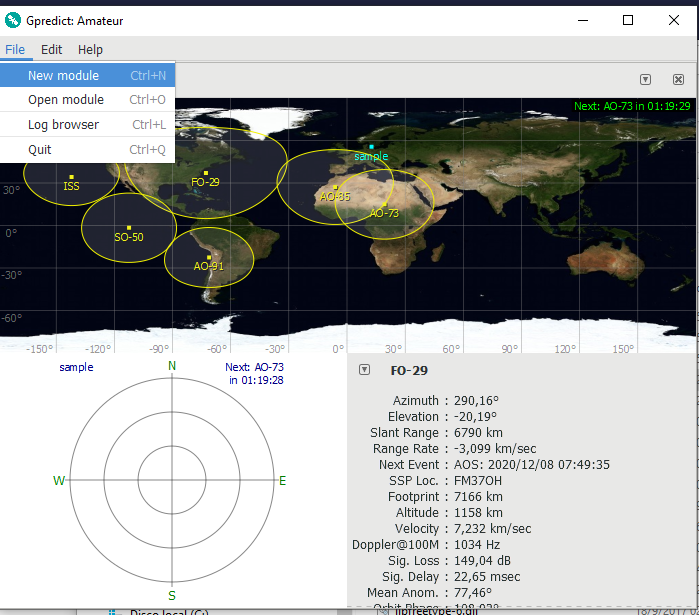
\includegraphics[width=\textwidth,height=8cm]{create_module}
	\caption{Creación de un módulo dentro de Gpredict} 
	\label{fig:create_modul_gpred}	
\end{figure}

Al realizar esto, se abre la ventana, dónde selecciona los satélites a seguir. Esta ventana se muestra en la figura \ref{fig:sel_sat}. En esta ventana, seleccionamos los satélites, y lo nombramos al módulo. En este caso, se lo denominamos arduino. 

\begin{figure}[ht]
	\centering
	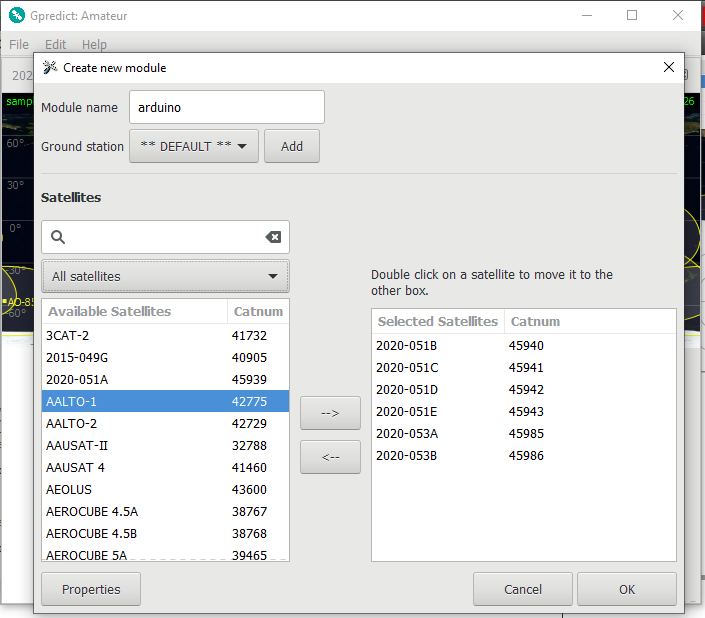
\includegraphics[height=10cm,width=\textwidth]{select_sat}
	\caption{Selección de satélites para el nuevo módulo creado} 
	\label{fig:sel_sat}	
\end{figure}
%\vspace{}
Donde dice ``Ground station'',se debe configurar latitud y longitud de la antena. Luego se presiona OK. Después de esto, ya se creó el módulo. Para abrirlo cuando desee, debe dirigirse a file $\rightarrow$ open module, y elegir ``arduino'' como módulo.
\subsection{Configuración del rotador en Gpredict} \label{subs:conf_Gpredict}
Para configurar el rotador, en la página que se abre al iniciar el programa(ver figura	\ref{fig:iu_gpredict}), debe dirigirse a edit $\rightarrow$ prefences. Al realizar esto, se abre la siguiente ventana: 
\begin{figure}[H]
	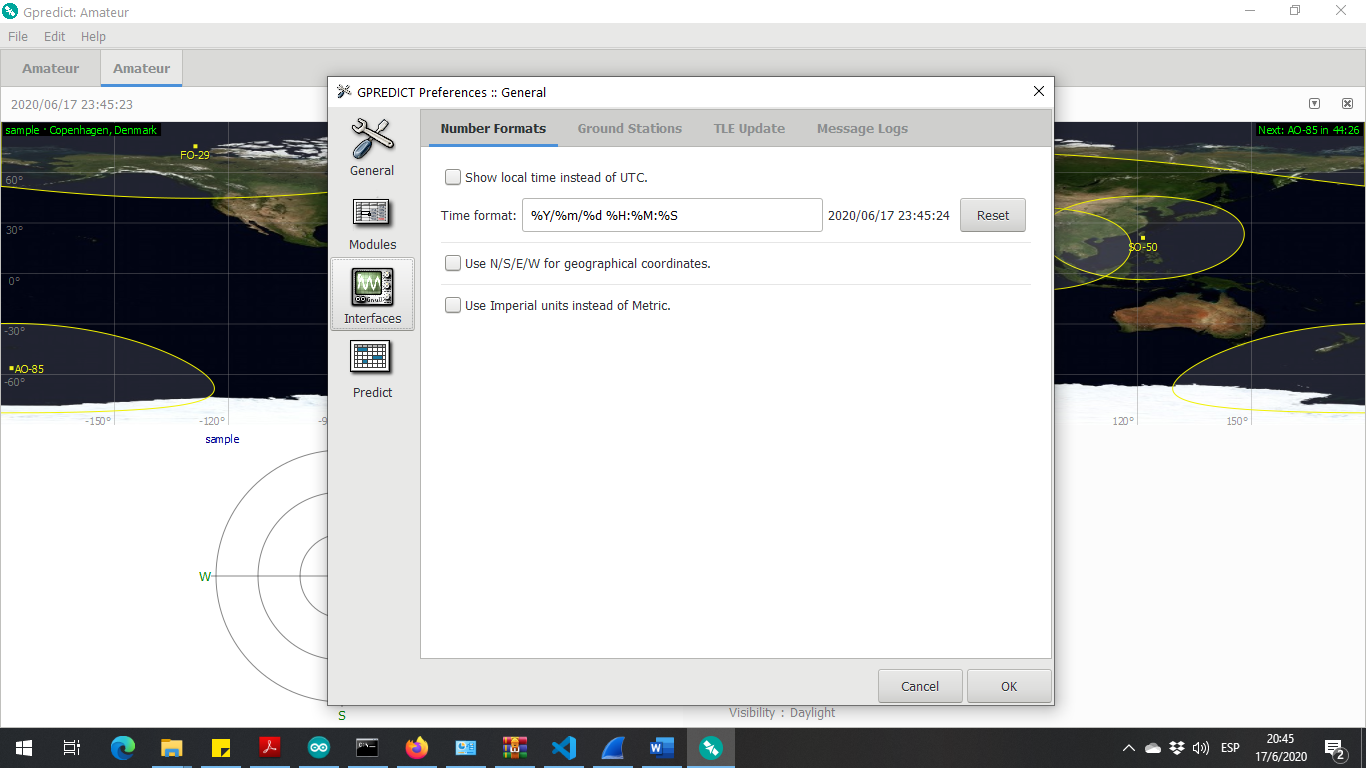
\includegraphics[height=5cm,width=\textwidth]{select_rot}
	\caption{Configuración de rotador}
%	\label{key}
\end{figure} 

Luego de esto, debe presionar en la parte izquierda de la figura anterior, donde dice ``interfaces''. Al realizar esto, debe presionar, en la pestaña ``rotators''. A continuación se la ventana que se abre al presionar sobre interfaces
\begin{figure}[H]
	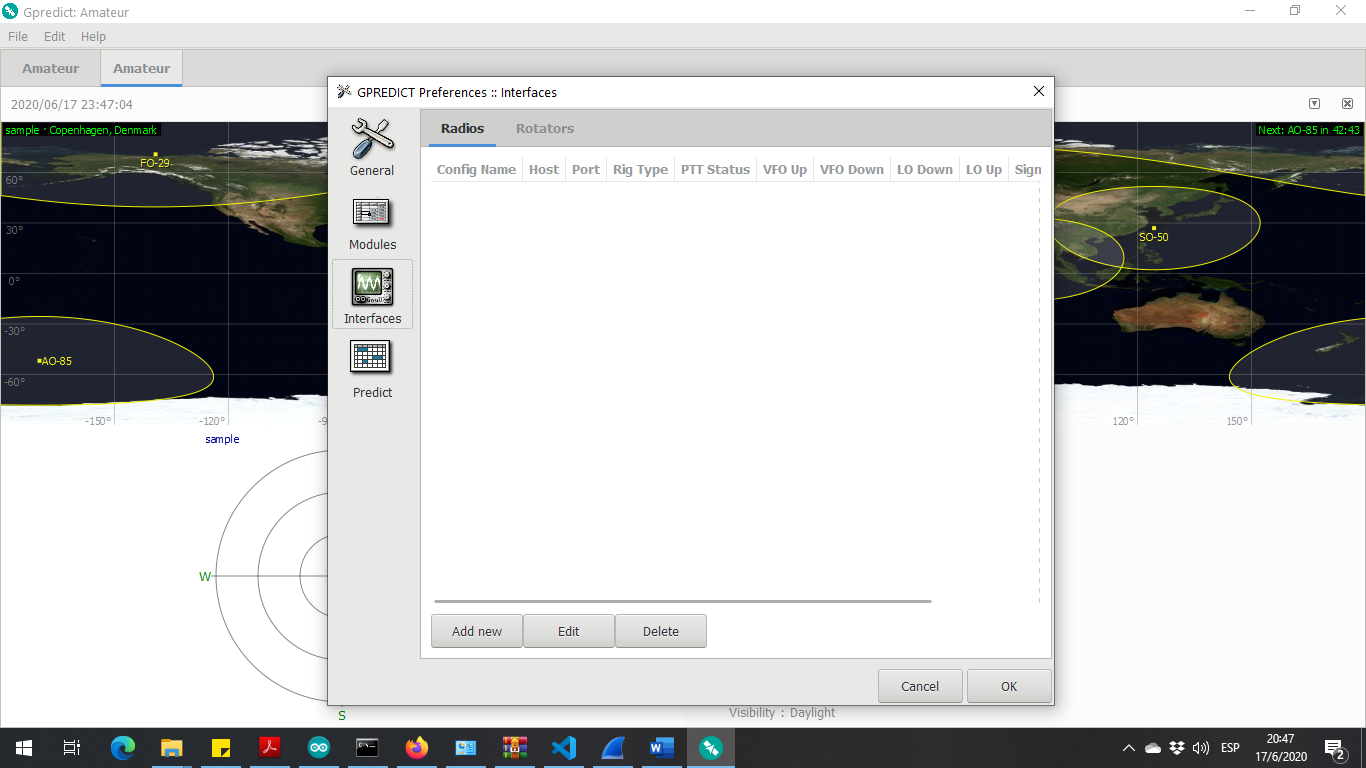
\includegraphics[height=10cm,width=\textwidth]{rotators_int}
	\caption{Configuración de rotador}
\end{figure} 

Luego, debe presionar en la pestaña rotators, y presionar donde dice ``add new'', y se abre una ventana como la que se muestra en la figura \ref{fig:conf_rot_ip}: 

\begin{figure}[h]
	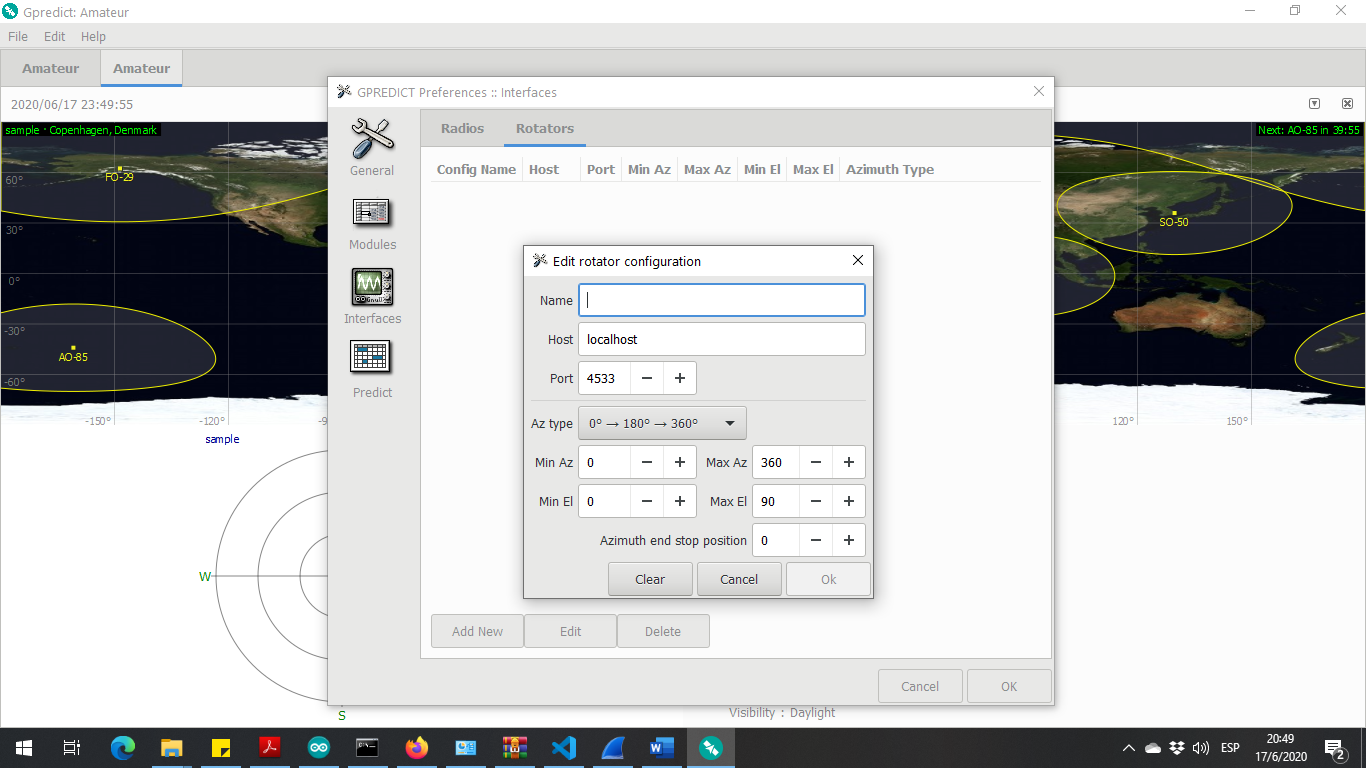
\includegraphics[height=8cm]{conf_rot}
	\caption{Configuración de rotador}
	\label{fig:conf_rot_ip}
\end{figure} 

Los parámetros a configurar son nombre del rotador(el que desee el usuario), ángulos máximos y mínimos de la antena. Estos parámetros se verán en el siguiente capítulo. Además, se observan que se debe definir el host y el puerto. El host, es la IP del dispositivo desarrollado en el presente documento, y el puerto, se define según el gusto del usuario, en nuestro caso, se va a utilizar el puerto por defecto (4533).Luego de rellenar los datos, debe seleccionar OK, y con esto, está configurado el rotador. Se pueden definir tantos rotadores como se deseen, se deben repetir los pasos. 

Una vez creado el rotador,para visualizar el rotador desde la pantalla principal, debe dirigirse a la parte derecha de la pantalla principal, y presionar ahí. En ese lugar, aparece un menú, debe dirigirse a ``antena control'', como se ve en la figura \ref{fig:ant_ctrl} 
\begin{figure}[H]
	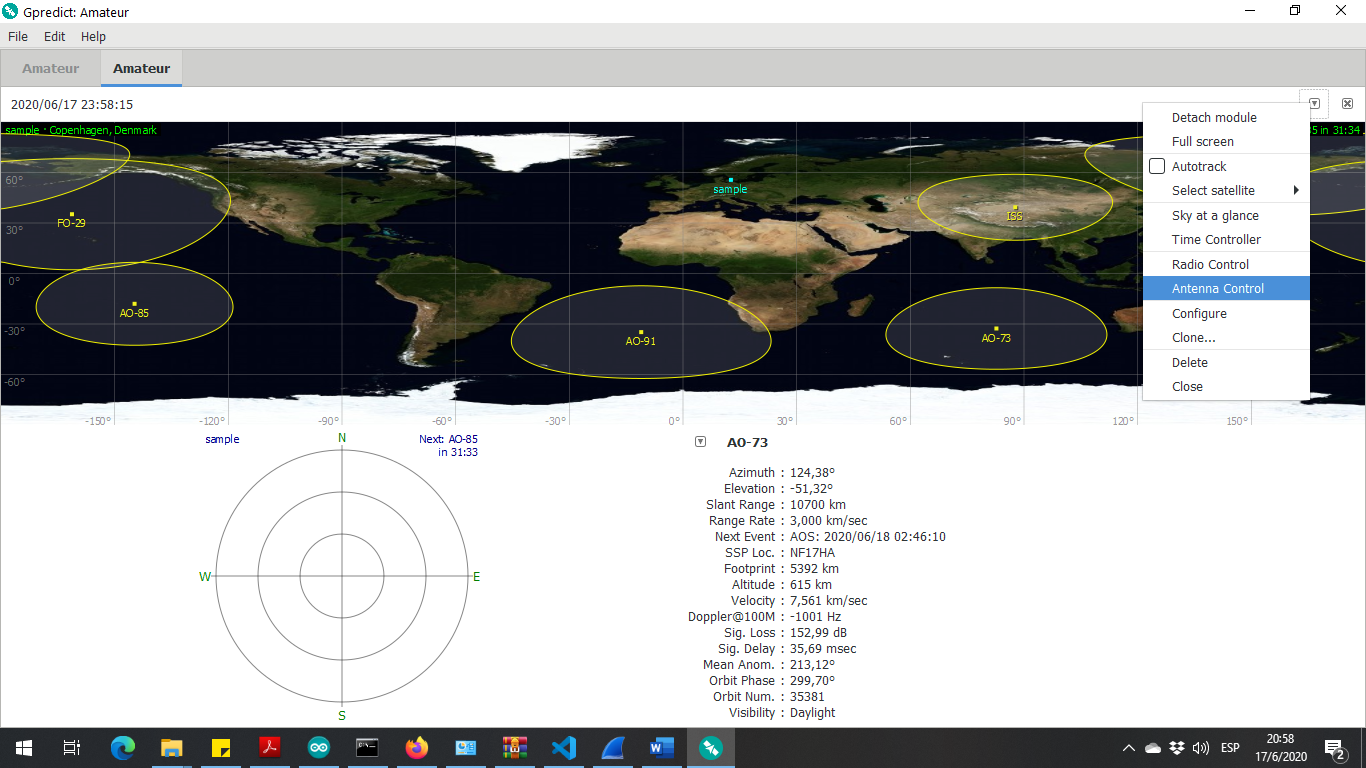
\includegraphics[height=10cm,width=\linewidth]{antena_control}
	\caption{Ver el rotador o rotadores configurados} 
	\label{fig:ant_ctrl}
\end{figure}



Al realizar este paso, aparece el rotador de antena, que se ve en la siguiente figura 

\begin{figure}[H]
	\centering 
	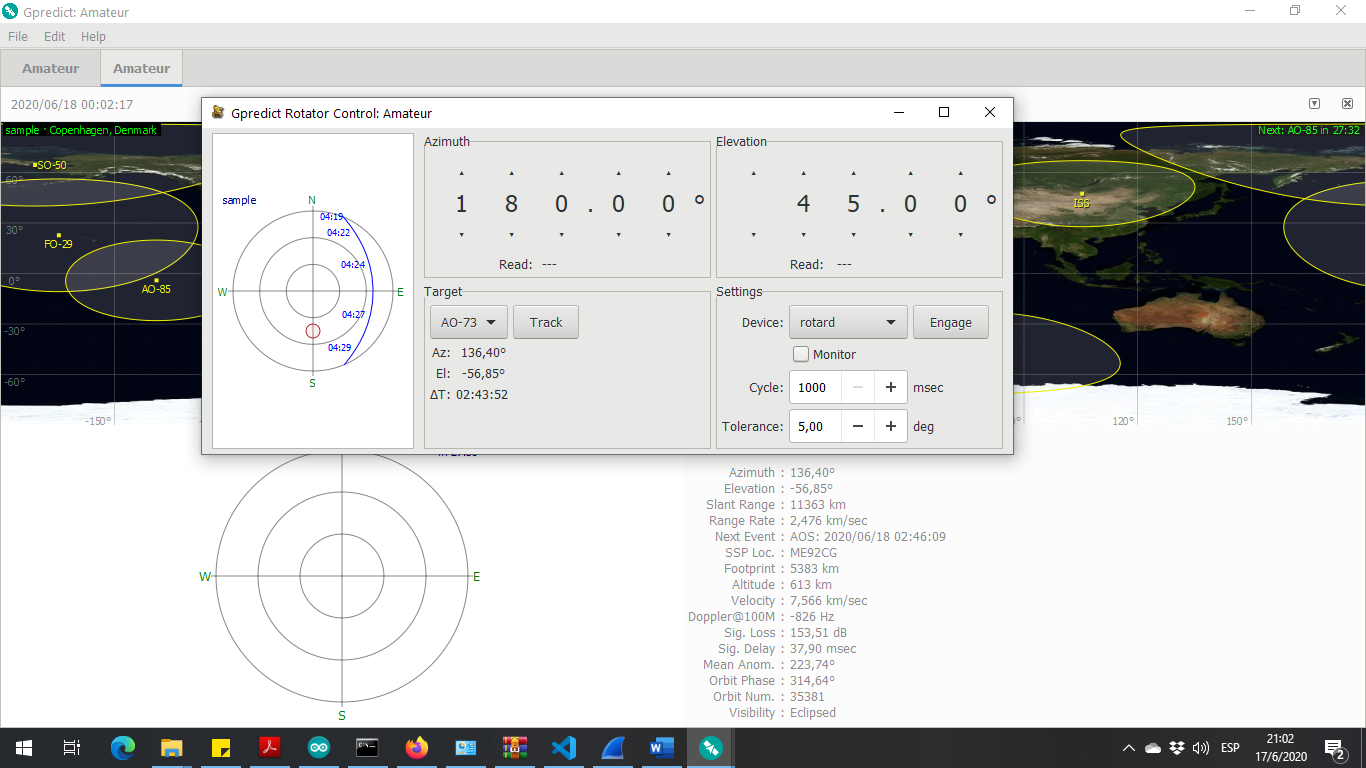
\includegraphics[trim=5.4cm 8cm 9.2cm 2.4cm ,clip,width=\linewidth,height=5cm]{antena_gpr_control}
	\caption{Panel de control del rotador de Gpredict} 
	\label{fig:pan_ctrl_antena}
\end{figure}

En esta figura, se observan dos botones, y dos menús, y un mapa de la antena. Estos dos botones son ``track'' y ``engage''. En el menú de track, realizamos el seguimiento automático. El menú, engage, sirve para realizar la calibración de la antena. El sistema de coordenadas empleado por este software es horizontal-azimutal, con el cero en el polo norte. Estas coordenadas son definidas en la fase 3, donde se muestra el análisis matemático de estas.  

Las medidas angulares, corresponden a los ángulos de la antena, estos se van a mostrar en el capítulo correspondiente a sistemas de coordenadas. Por ahora, solo basta con conocer la interfaz, luego se ajustan los detalles, para configurar el Gpredict, en base a la antena que tiene la institución, ajustando ángulos y límites de la misma. Esto se realiza en la fase 3, donde se van a mostrar los sistemas de coordenadas, y las relaciones entre ellos. En el próximo capítulo, se muestra cómo debe realizarse el seguimiento de satélites, mediante la comunicación con el dispositivo desarrollado en este documento. 



 
\section{Software Stellarium} 


Este programa, es libre, y está pensado en el apuntamiento de telescopios. Posee seguimiento de estrellas y satélites. Debido a que el apuntamiento de los telescopios, y/o antenas, depende de la posición del observador en la tierra, se debe configurar la posición geográfica dentro del software, para que se pueda realizar el apuntamiento de forma correcta. Para elegir la posición, dentro del software stellarium, oprimiendo el boton F6 o moviendo el cursor del mouse hacia la izquierda, y seleccionando posición, se abre la siguiente ventana de configuración: 
\begin{figure}[ht]
	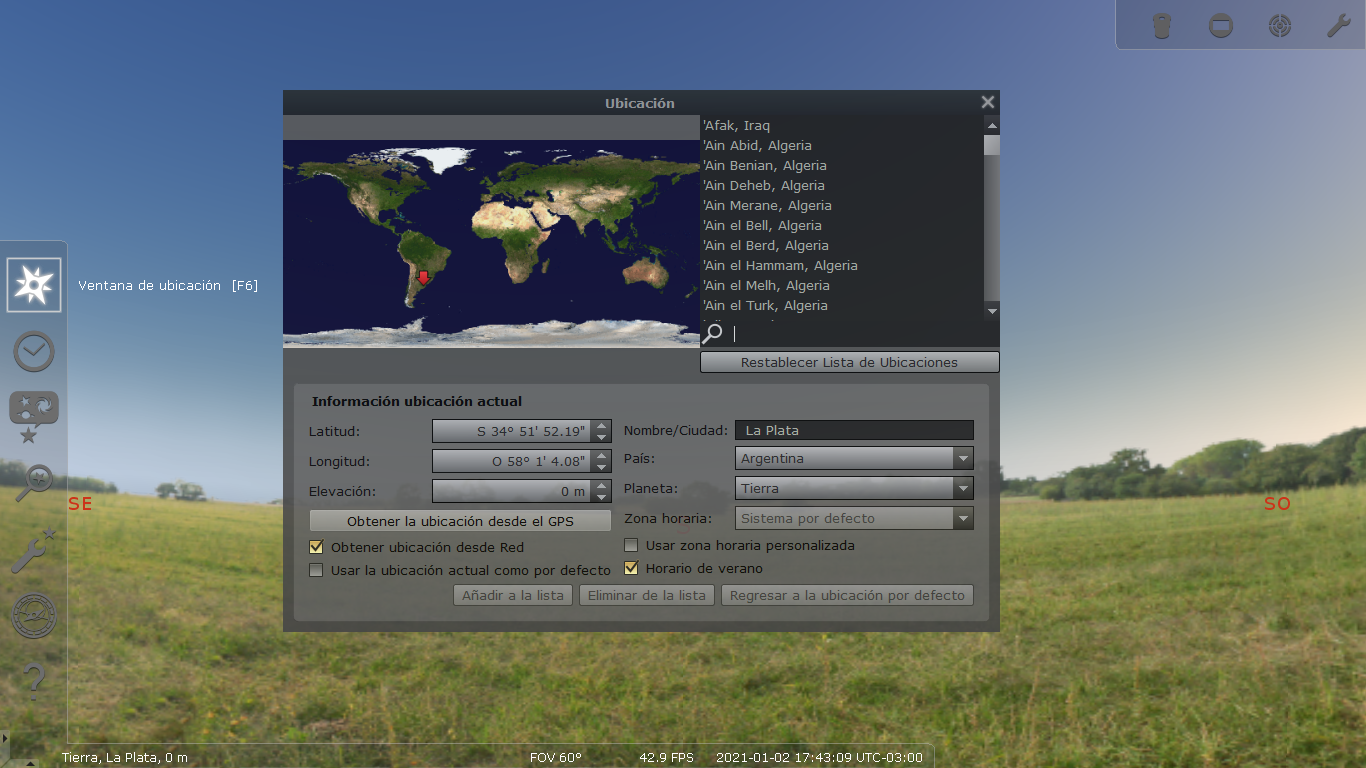
\includegraphics[width=\textwidth]{stel_sel_pos} 
	\caption{configuración de coordenadas locales dentro de stellarium} 
	\label{fig:stell_poss_conf}
\end{figure}

En esa ventana, debe seleccionarse, la latitud, longitud y altitud del lugar en el que se encuentra el telescopio o antena. Esta guía ha sido basada en la referencia \cite{mgpredict}, que es el manual oficial del software. 

\subsection{Configuración de la red en Stellarium} \label{sub:conf_stellarium_red}


Para poder conectar una PC de la institución, con el dispositivo, debe configurar el puerto(o socket) con el cual se intercambiarán mensajes, y la dirección IP del dispositivo receptor, que será el encargado de mover la antena o telescopio. Para configurar el telescopio, debe dirigirse a configuración, luego presionar en la pestaña pluggins, y en la parte izquierda seleccionar ``control del telescopio''. A continuación se deja la imagen de este proceso: 
 
\begin{figure}[h]
	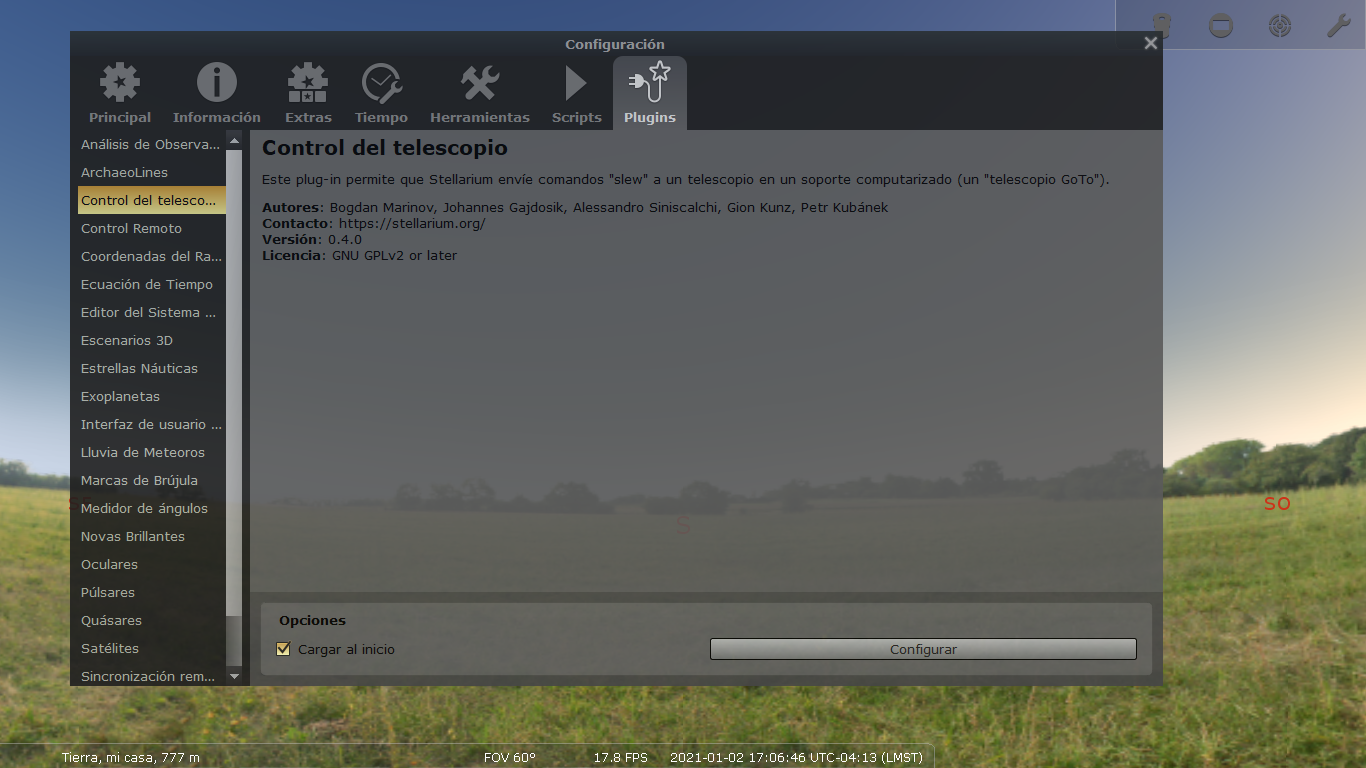
\includegraphics[width=\textwidth]{conf_tel_red1} 
	\caption{configuración de coordenadas locales dentro de stellarium} 
	\label{fig:stell_conf_red}
\end{figure}

Una vez, en esta ventana, se debe seleccionar el botón ``configurar'', debajo a la izquierda de esta ventana, y luego, se abre una ventana cómo la que se muestra a continuación. 

\begin{figure}[H]
	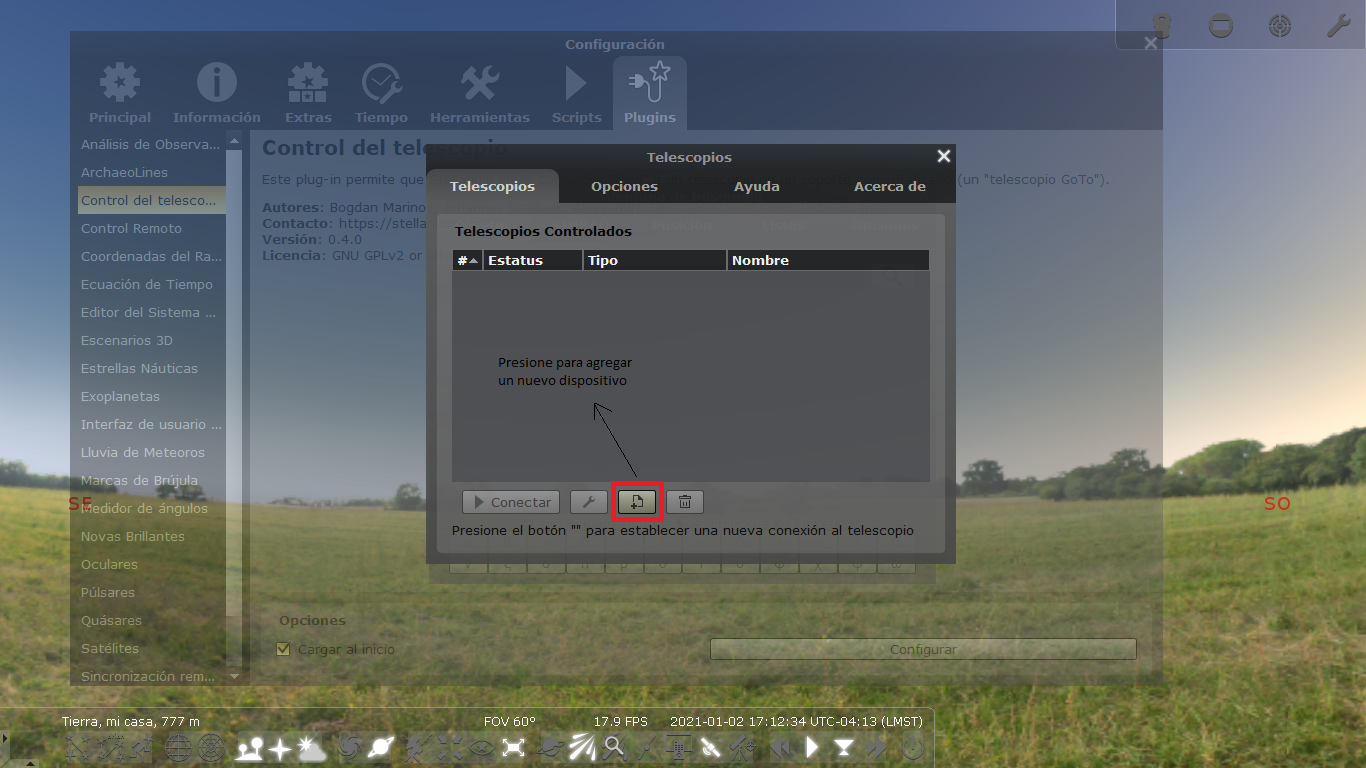
\includegraphics[height=10cm,width=\textwidth]{stell_conf_red_2} 
	\caption{configuración de coordenadas locales dentro de stellarium} 
	\label{fig:stell_conf_red_2}
\end{figure}

Luego, debe presionar donde muestra la imagen anterior para empezar a agregar el primer dispositivo. Se realiza un click sobre el símbolo recuadrado en rojo de la figura anterior, se abre la siguiente ventana, donde deben elegirse los parámetros para configurar el dispositivo hacia cual enviará los datos.
%\begin{wrapfigure}[21]{l}{0.4\textwidth}
\begin{figure}
	\centering
	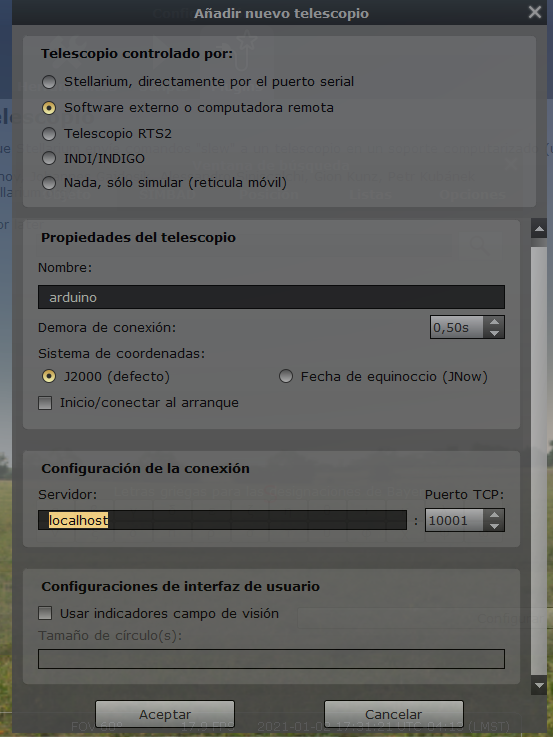
\includegraphics[scale=0.5]{stellarium-024}
	\caption{Ventana de configuración de red del software Stellarium.}
\end{figure} 
Donde dice ``localhost'',debe introducirse la IP del dispositivo que es capaz de realizar el movimiento de la antena, el nombre, es a elección del usuario, y hay dos tipos de coordenadas: J2000 y fecha de equinoccio. Estas coordenadas están relacionadas con la selección de la referencia para las coordenadas ecuatoriales. Estas se discuten en \ref{cap:sist_cord}. Se elige J2000.

Una vez configurado el dispositivo, queda por intentar entender el protocolo, que éste emplea para comunicarse con los dispositivos. Si desea conocer más opciones de este programa, puede ver la referencia \cite{stellman}

\subsection{Protocolo de comunicación Stellarium} \label{sub:comun_stell}
El stellarium, no es capaz de recibir datos en este modo de configuración (al menos, por lo investigado hasta el momento), pero si es capaz de enviar datos al dispositivo conectado en la red. Este emplea dos números binarios, uno para cada eje. Según su documentación, al configurar un dispositivo, este invoca a un programa denominado ``telescope server'', el cual trabaja sobre TCP/IP. Este, es el que envía las coordenadas al dispositivo. Los mensajes se basan en bytes, donde están agrupados del siguiente modo: 

\begin{itemize}
	\item LENGTH : 2 bytes - Indica la longitud total del mensaje
	\item TIME : 8 bytes. Tiempo UT a partir de 01/01/1970 en microsegundos. Actualmente en desuso 
	\item RA: 4 bytes(sin signo) - ascensión recta: 
	\item DEC : 4 bytes,con signo
	\item status: 4bytes con signo. Si status = 0 -> OK, si status<0 hay algún error.  
\end{itemize}

Cabe destacar, que internet, o las redes, son protocolos big-endian, mientras que el microcontrolador atMEGA328p(arduino UNO) es little-endian. Esto se debe solucionar reordenando los bits de llegada hacia el dispositivo. Además, debe realizar una transformación de coordenadas para poder realizar el apuntamiento de la antena. 

